\documentclass{standalone}
\usepackage{tikz}
\usetikzlibrary{patterns, positioning}
\usepackage[sfdefault]{ClearSans} %% option 'sfdefault' activates Clear Sans as the default text font
\usepackage[T1]{fontenc}

\begin{document}
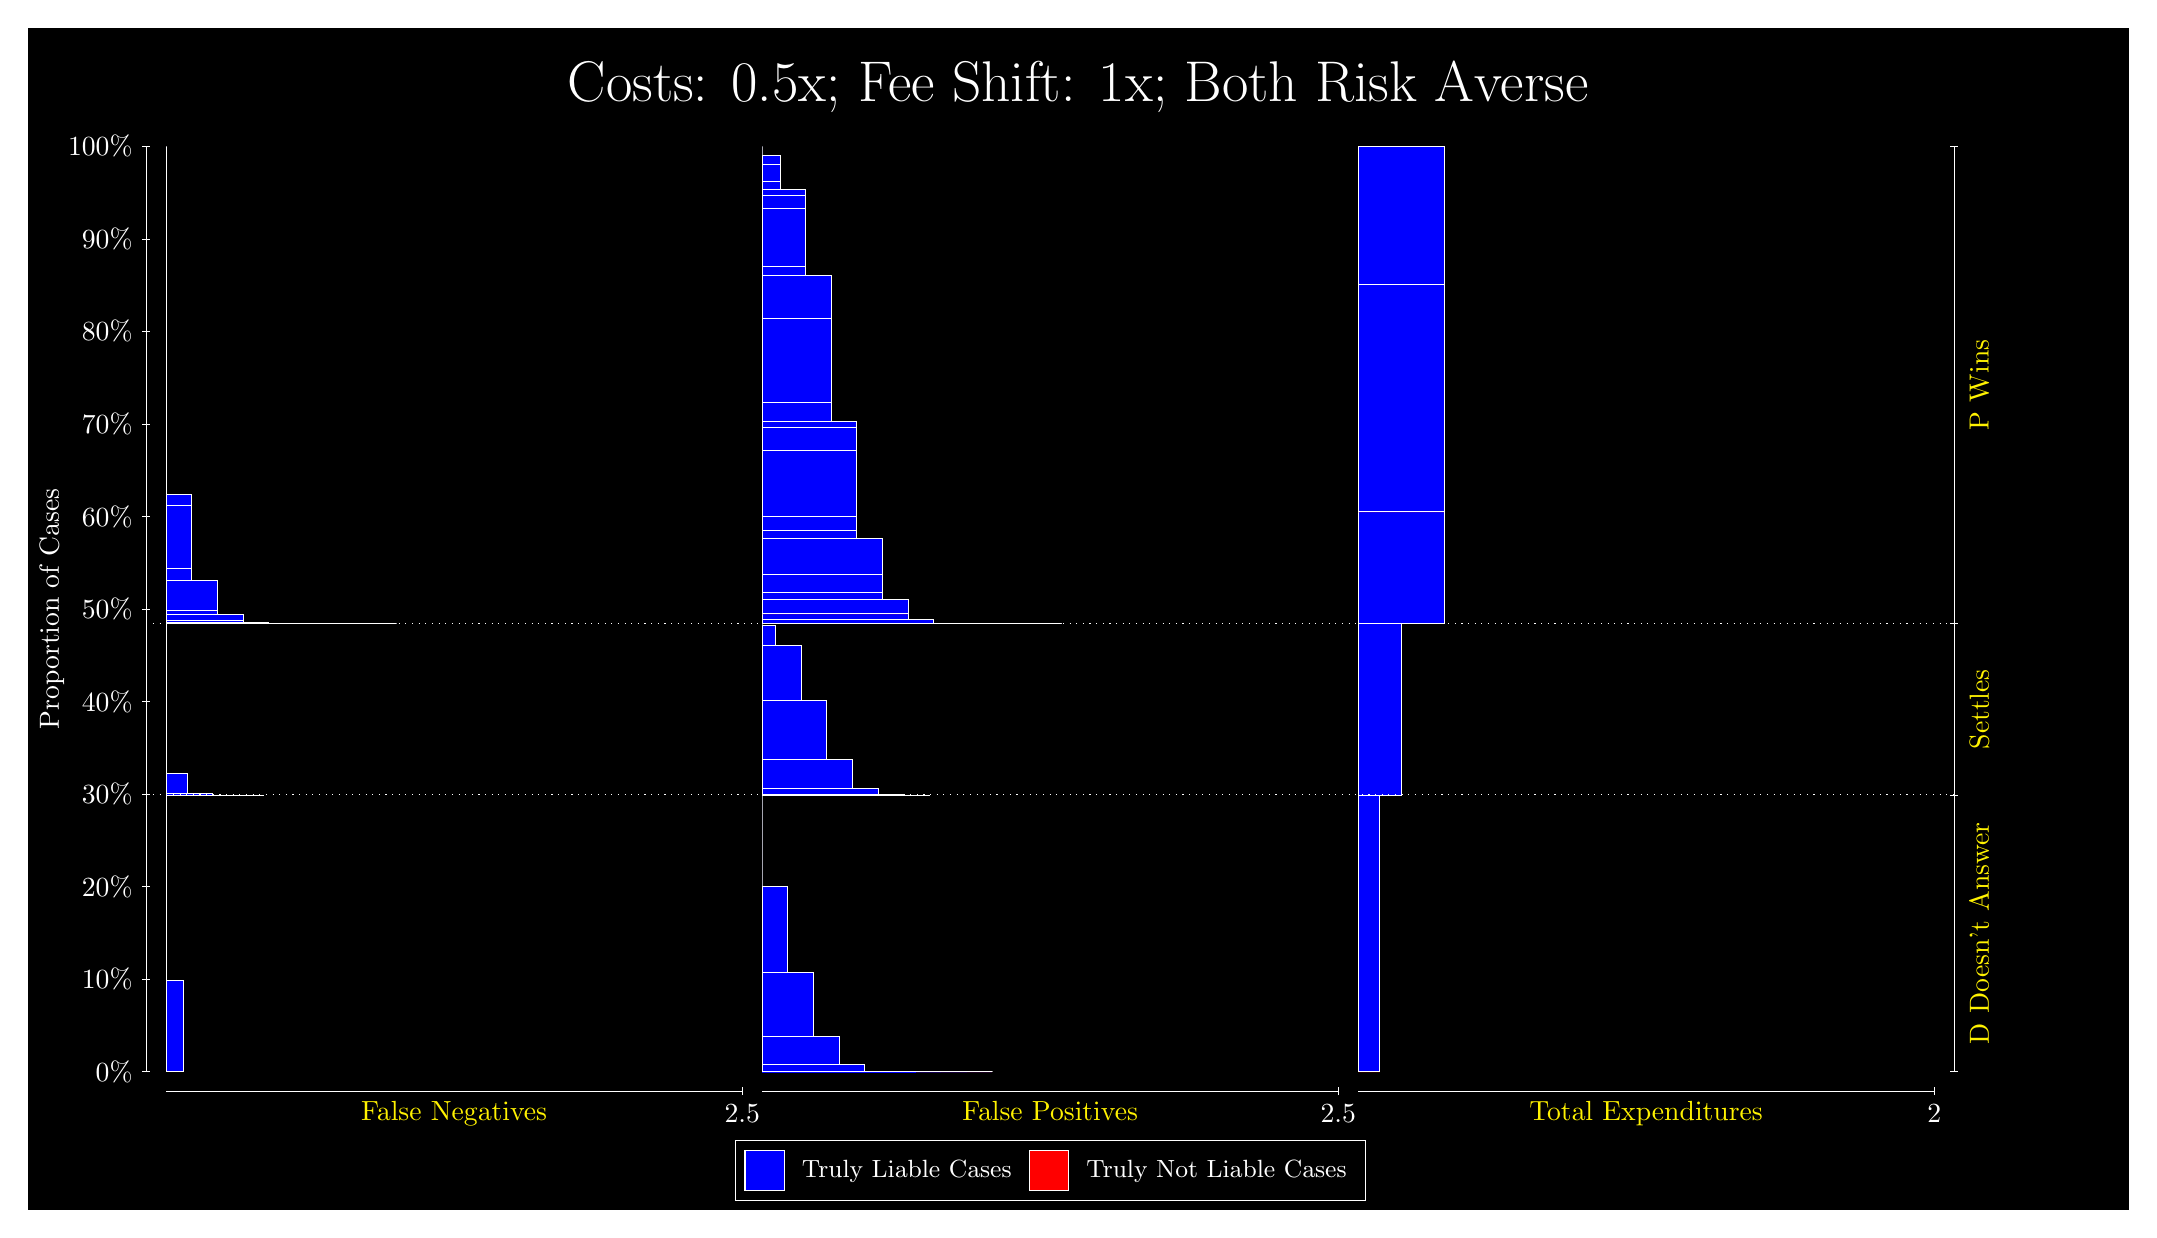
\begin{tikzpicture}
\draw[fill=black] (0,0) rectangle (26.667,15);
\draw[text=white] (0,13.5) rectangle (26.667,15) node[midway] {\huge Costs: 0.5x; Fee Shift: 1x; Both Risk Averse};
\draw[white, very thin] (1.5,1.75) -- (1.5,13.5);
\node[rotate=90, text=white, anchor=center] at (0.3, 7.625) {Proportion of Cases};
\draw[white, very thin] (1.45,1.75) -- (1.55,1.75);
\node[text=white, anchor=east] at (1.45, 1.75) {0\%};
\draw[white, very thin] (1.45,2.925) -- (1.55,2.925);
\node[text=white, anchor=east] at (1.45, 2.925) {10\%};
\draw[white, very thin] (1.45,4.1) -- (1.55,4.1);
\node[text=white, anchor=east] at (1.45, 4.1) {20\%};
\draw[white, very thin] (1.45,5.275) -- (1.55,5.275);
\node[text=white, anchor=east] at (1.45, 5.275) {30\%};
\draw[white, very thin] (1.45,6.45) -- (1.55,6.45);
\node[text=white, anchor=east] at (1.45, 6.45) {40\%};
\draw[white, very thin] (1.45,7.625) -- (1.55,7.625);
\node[text=white, anchor=east] at (1.45, 7.625) {50\%};
\draw[white, very thin] (1.45,8.8) -- (1.55,8.8);
\node[text=white, anchor=east] at (1.45, 8.8) {60\%};
\draw[white, very thin] (1.45,9.975) -- (1.55,9.975);
\node[text=white, anchor=east] at (1.45, 9.975) {70\%};
\draw[white, very thin] (1.45,11.15) -- (1.55,11.15);
\node[text=white, anchor=east] at (1.45, 11.15) {80\%};
\draw[white, very thin] (1.45,12.325) -- (1.55,12.325);
\node[text=white, anchor=east] at (1.45, 12.325) {90\%};
\draw[white, very thin] (1.45,13.5) -- (1.55,13.5);
\node[text=white, anchor=east] at (1.45, 13.5) {100\%};

\draw[white, very thin] (24.457,1.75) -- (24.457,13.5);
\draw[white, very thin] (24.407,1.75) -- (24.507,1.75);
\node[anchor=west] at (24.407, 1.75) {};
\draw[white, very thin] (24.407,5.264) -- (24.507,5.264);
\node[anchor=west] at (24.407, 5.264) {};
\draw[white, very thin] (24.407,7.4401) -- (24.507,7.4401);
\node[anchor=west] at (24.407, 7.4401) {};
\draw[white, very thin] (24.407,13.5) -- (24.507,13.5);
\node[anchor=west] at (24.407, 13.5) {};

\draw[white, very thin, fill=blue] (1.75,1.75) rectangle (1.9696,2.9145);
\draw[white, very thin, fill=red] (1.75,2.9145) rectangle (1.75,2.9145);
\draw[white, very thin, fill=blue] (1.75,2.9145) rectangle (1.75,5.264);
\draw[white, very thin, fill=blue] (1.75,5.264) rectangle (2.9942,5.264);
\draw[white, very thin, fill=blue] (1.75,5.264) rectangle (2.6689,5.2646);
\draw[white, very thin, fill=blue] (1.75,5.2646) rectangle (2.3436,5.2891);
\draw[white, very thin, fill=blue] (1.75,5.2891) rectangle (2.0184,5.5376);
\draw[white, very thin, fill=red] (1.75,5.5376) rectangle (1.75,5.5376);
\draw[white, very thin, fill=blue] (1.75,5.5376) rectangle (1.75,7.4401);
\draw[white, very thin, fill=blue] (1.75,7.4401) rectangle (4.6775,7.4401);
\draw[white, very thin, fill=blue] (1.75,7.4401) rectangle (4.3523,7.4401);
\draw[white, very thin, fill=blue] (1.75,7.4401) rectangle (4.027,7.4402);
\draw[white, very thin, fill=blue] (1.75,7.4402) rectangle (4.027,7.4402);
\draw[white, very thin, fill=blue] (1.75,7.4402) rectangle (3.7017,7.4402);
\draw[white, very thin, fill=blue] (1.75,7.4402) rectangle (3.7017,7.4403);
\draw[white, very thin, fill=blue] (1.75,7.4403) rectangle (3.3764,7.442);
\draw[white, very thin, fill=blue] (1.75,7.442) rectangle (3.0511,7.4484);
\draw[white, very thin, fill=blue] (1.75,7.4484) rectangle (3.0511,7.4577);
\draw[white, very thin, fill=blue] (1.75,7.4577) rectangle (2.7258,7.4869);
\draw[white, very thin, fill=blue] (1.75,7.4869) rectangle (2.7258,7.5556);
\draw[white, very thin, fill=blue] (1.75,7.5556) rectangle (2.7258,7.5593);
\draw[white, very thin, fill=blue] (1.75,7.5593) rectangle (2.4006,7.6029);
\draw[white, very thin, fill=blue] (1.75,7.6029) rectangle (2.4006,7.9836);
\draw[white, very thin, fill=blue] (1.75,7.9836) rectangle (2.0753,8.1453);
\draw[white, very thin, fill=blue] (1.75,8.1453) rectangle (2.0753,8.9417);
\draw[white, very thin, fill=blue] (1.75,8.9417) rectangle (2.0753,9.0827);
\draw[white, very thin, fill=red] (1.75,9.0827) rectangle (1.75,9.0827);
\draw[white, very thin, fill=blue] (1.75,9.0827) rectangle (1.75,13.5);
\draw[white, very thin, fill=red] (9.3189,1.75) rectangle (12.246,1.75);
\draw[white, very thin, fill=blue] (9.3189,1.75) rectangle (12.246,1.75);
\draw[white, very thin, fill=blue] (9.3189,1.75) rectangle (11.921,1.75);
\draw[white, very thin, fill=blue] (9.3189,1.75) rectangle (11.596,1.75);
\draw[white, very thin, fill=blue] (9.3189,1.75) rectangle (11.271,1.7503);
\draw[white, very thin, fill=blue] (9.3189,1.7503) rectangle (10.945,1.7576);
\draw[white, very thin, fill=blue] (9.3189,1.7576) rectangle (10.62,1.8361);
\draw[white, very thin, fill=blue] (9.3189,1.8361) rectangle (10.295,2.1984);
\draw[white, very thin, fill=blue] (9.3189,2.1984) rectangle (9.9694,3.0086);
\draw[white, very thin, fill=blue] (9.3189,3.0086) rectangle (9.6442,4.0995);
\draw[white, very thin, fill=blue] (9.3189,4.0995) rectangle (9.3189,5.264);
\draw[white, very thin, fill=red] (9.3189,5.264) rectangle (11.441,5.264);
\draw[white, very thin, fill=blue] (9.3189,5.264) rectangle (11.441,5.2644);
\draw[white, very thin, fill=blue] (9.3189,5.2644) rectangle (11.116,5.2722);
\draw[white, very thin, fill=blue] (9.3189,5.2722) rectangle (10.791,5.3512);
\draw[white, very thin, fill=blue] (9.3189,5.3512) rectangle (10.465,5.7113);
\draw[white, very thin, fill=blue] (9.3189,5.7113) rectangle (10.14,6.4626);
\draw[white, very thin, fill=blue] (9.3189,6.4626) rectangle (9.8149,7.1665);
\draw[white, very thin, fill=blue] (9.3189,7.1665) rectangle (9.4896,7.4151);
\draw[white, very thin, fill=blue] (9.3189,7.4151) rectangle (9.3189,7.4401);
\draw[white, very thin, fill=red] (9.3189,7.4401) rectangle (13.125,7.4401);
\draw[white, very thin, fill=blue] (9.3189,7.4401) rectangle (13.125,7.4401);
\draw[white, very thin, fill=red] (9.3189,7.4401) rectangle (12.799,7.4401);
\draw[white, very thin, fill=blue] (9.3189,7.4401) rectangle (12.799,7.4401);
\draw[white, very thin, fill=blue] (9.3189,7.4401) rectangle (12.474,7.4402);
\draw[white, very thin, fill=red] (9.3189,7.4402) rectangle (12.474,7.4402);
\draw[white, very thin, fill=blue] (9.3189,7.4402) rectangle (12.474,7.4402);
\draw[white, very thin, fill=blue] (9.3189,7.4402) rectangle (12.149,7.4403);
\draw[white, very thin, fill=blue] (9.3189,7.4403) rectangle (12.149,7.4404);
\draw[white, very thin, fill=red] (9.3189,7.4404) rectangle (12.149,7.4404);
\draw[white, very thin, fill=blue] (9.3189,7.4404) rectangle (12.149,7.4408);
\draw[white, very thin, fill=red] (9.3189,7.4408) rectangle (11.824,7.4408);
\draw[white, very thin, fill=blue] (9.3189,7.4408) rectangle (11.824,7.4446);
\draw[white, very thin, fill=blue] (9.3189,7.4446) rectangle (11.824,7.446);
\draw[white, very thin, fill=blue] (9.3189,7.446) rectangle (11.824,7.4477);
\draw[white, very thin, fill=red] (9.3189,7.4477) rectangle (11.498,7.4477);
\draw[white, very thin, fill=blue] (9.3189,7.4477) rectangle (11.498,7.489);
\draw[white, very thin, fill=blue] (9.3189,7.489) rectangle (11.498,7.4988);
\draw[white, very thin, fill=blue] (9.3189,7.4988) rectangle (11.173,7.5641);
\draw[white, very thin, fill=red] (9.3189,7.5641) rectangle (11.173,7.5641);
\draw[white, very thin, fill=blue] (9.3189,7.5641) rectangle (11.173,7.7496);
\draw[white, very thin, fill=blue] (9.3189,7.7496) rectangle (10.848,7.8408);
\draw[white, very thin, fill=blue] (9.3189,7.8408) rectangle (10.848,8.0712);
\draw[white, very thin, fill=red] (9.3189,8.0712) rectangle (10.848,8.0712);
\draw[white, very thin, fill=blue] (9.3189,8.0712) rectangle (10.848,8.5213);
\draw[white, very thin, fill=blue] (9.3189,8.5213) rectangle (10.522,8.6301);
\draw[white, very thin, fill=blue] (9.3189,8.6301) rectangle (10.522,8.8035);
\draw[white, very thin, fill=red] (9.3189,8.8035) rectangle (10.522,8.8035);
\draw[white, very thin, fill=blue] (9.3189,8.8035) rectangle (10.522,9.6342);
\draw[white, very thin, fill=blue] (9.3189,9.6342) rectangle (10.522,9.9266);
\draw[white, very thin, fill=blue] (9.3189,9.9266) rectangle (10.522,10.01);
\draw[white, very thin, fill=blue] (9.3189,10.01) rectangle (10.197,10.251);
\draw[white, very thin, fill=red] (9.3189,10.251) rectangle (10.197,10.251);
\draw[white, very thin, fill=blue] (9.3189,10.251) rectangle (10.197,11.315);
\draw[white, very thin, fill=blue] (9.3189,11.315) rectangle (10.197,11.857);
\draw[white, very thin, fill=blue] (9.3189,11.857) rectangle (9.8718,11.978);
\draw[white, very thin, fill=blue] (9.3189,11.978) rectangle (9.8718,12.708);
\draw[white, very thin, fill=blue] (9.3189,12.708) rectangle (9.8718,12.881);
\draw[white, very thin, fill=blue] (9.3189,12.881) rectangle (9.8718,12.957);
\draw[white, very thin, fill=blue] (9.3189,12.957) rectangle (9.5466,13.059);
\draw[white, very thin, fill=blue] (9.3189,13.059) rectangle (9.5466,13.278);
\draw[white, very thin, fill=blue] (9.3189,13.278) rectangle (9.5466,13.381);
\draw[white, very thin, fill=blue] (9.3189,13.381) rectangle (9.3189,13.5);
\draw[white, very thin, fill=red] (16.888,1.75) rectangle (17.162,1.75);
\draw[white, very thin, fill=blue] (16.888,1.75) rectangle (17.162,5.264);
\draw[white, very thin, fill=red] (16.888,5.264) rectangle (17.437,5.264);
\draw[white, very thin, fill=blue] (16.888,5.264) rectangle (17.437,7.4401);
\draw[white, very thin, fill=red] (16.888,7.4401) rectangle (17.986,7.4401);
\draw[white, very thin, fill=blue] (16.888,7.4401) rectangle (17.986,8.8601);
\draw[white, very thin, fill=red] (16.888,8.8601) rectangle (17.986,8.8601);
\draw[white, very thin, fill=blue] (16.888,8.8601) rectangle (17.986,11.749);
\draw[white, very thin, fill=red] (16.888,11.749) rectangle (17.986,11.749);
\draw[white, very thin, fill=blue] (16.888,11.749) rectangle (17.986,13.5);
\draw[white, dotted] (1.5,5.264) -- (24.457,5.264);
\draw[white, dotted] (1.5,7.4401) -- (24.457,7.4401);
\draw[white, very thin] (1.75,1.5) -- (9.0689,1.5);
\node[text=yellow, anchor=north] at (5.4094, 1.5) {False Negatives};
\draw[white, very thin] (9.0689,1.45) -- (9.0689,1.55);
\node[text=white, anchor=north] at (9.0689, 1.45) {2.5};

\draw[white, very thin] (9.3189,1.5) -- (16.638,1.5);
\node[text=yellow, anchor=north] at (12.978, 1.5) {False Positives};
\draw[white, very thin] (16.638,1.45) -- (16.638,1.55);
\node[text=white, anchor=north] at (16.638, 1.45) {2.5};

\draw[white, very thin] (16.888,1.5) -- (24.207,1.5);
\node[text=yellow, anchor=north] at (20.547, 1.5) {Total Expenditures};
\draw[white, very thin] (24.207,1.45) -- (24.207,1.55);
\node[text=white, anchor=north] at (24.207, 1.45) {2};

\node[text=yellow, centered, rotate=90] at (24.777, 3.507) {D Doesn't Answer};
\node[text=yellow, centered, rotate=90] at (24.777, 6.3521) {Settles};
\node[text=yellow, centered, rotate=90] at (24.777, 10.47) {P Wins};

\draw (12.978300999999998,1.5) node[draw=none] (baseCoordinate) {};
\begin{scope}[align=center]
        \matrix[scale=0.5, draw=white, below=0.5cm of baseCoordinate, nodes={draw}, column sep=0.1cm]{
            \node[rectangle, draw, minimum width=0.5cm, minimum height=0.5cm, fill=blue] {}; &
            \node[draw=none, font=\small, text=white] (B) {Truly Liable Cases}; &
            \node[rectangle, draw, minimum width=0.5cm, minimum height=0.5cm, fill=red] {}; &
            \node[draw=none, font=\small, text=white] (B) {Truly Not Liable Cases}; \\
            };
\end{scope}

\end{tikzpicture}
\end{document}